%%%% fatec-article.tex, 2024/03/10

\documentclass[
  a4paper,%% Tamanho de papel: a4paper, letterpaper (^), etc.
  12pt,%% Tamanho de fonte: 10pt (^), 11pt, 12pt, etc.
  english,%% Idioma secundário (penúltimo) (>)
  brazilian,%% Idioma primário (último) (>)
]{article}

%% Pacotes utilizados
\usepackage[]{fatec-article}
\usepackage{float}

%% Início do documento
\begin{document}
\vspace{8cm}
\begin{center}
    \large \textbf{\title{ARTEFATOS DO PROJETO DE SOFTWARE}}
\end{center}

\maketitle

\break

\tableofcontents

\break


%exemplo da forma de organização das seções e subseções, você deverá adaptar o template para a realidade do seu projeto.

\section*{Diagramas UML}
    Nesta seção serão apresentados os diagramas da UML utilizados para a modelagem do sistema desenvolvido. Dentre os diagramas utilizados, pode-se citar: Diagrama de Caso de Uso, Diagrama de Classe e Diagrama de Objetos.
    
    \subsection*{Diagrama de Caso de Uso}
    \addcontentsline{toc}{section}{Diagrama de Caso de Uso}

    Esse é um exemplo de diagrama de caso de uso, você deverá descrever todos os componentes presentes no diagrama (atores e funcionalidades do sistema).

\begin{figure}[H]
\centering
\caption{Diagrama de caso de uso}%
\label{fig:caso-de-uso}
 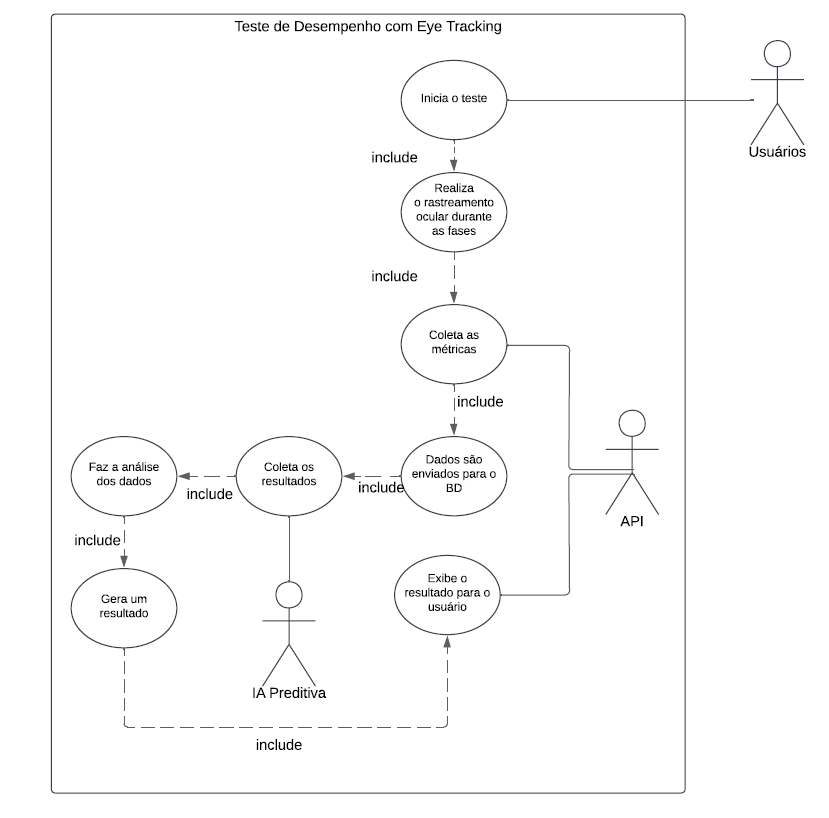
\includegraphics[width=1.1\textwidth]{Logos/caso-de-uso.png}
\SourceOrNote{Do próprio autor (2025)}
\end{figure}

    Não deixe a seção terminar com a imagem então sempre adicione um texto após a mesma.
    
    \subsection*{Diagrama de Classe}
    \addcontentsline{toc}{section}{Diagrama de Classe}

    Este Diagrama de Classe modela a estrutura de dados e as principais entidades do sistema de rastreamento ocular para avaliação de atenção.
    O diagrama ilustra quatro classes principais: Usuário, que armazena dados básicos de identificação, como nome, idade e sexo, além disso, contém os métodos logar(), logout(), jogar() e visualizarPréDiagnóstico(). A classe denominada Fases, que define as carcterísticas de cada fase do jogo, incluindo atributos como nome da fase (podendo variar entre "Fase 1", "Fase 2" e "Fase 3"), descrição, tempoTotal e o tipoAtençãoAvaliada. O método para esta classe é o iniciar() para começar uma fase do jogo. Possui a classe de Inteligência Aritifical (IA), que armazena os resultados brutos do rastreamento ocular, como dataTeste, usuário, métricas de foco (TempoInícioFoco, tempoMínimoFoco, tempoTotal, acertos), e contagens de erros (errosPorOmissão, errosPorComissão) todos como inteiros. A IA é responsável pelo processamento dos resultados e diagnóstico através dos métodos analisarResultados() e gerarPréDiagnóstico(). Por fim, a classe PréDiagnóstico que guarda o resultado final da avaliação de atenção para um usuário em uma determinada fase, incluindo usuário, fase, comentário e um valor de precisão. O pré diagnóstico é exibido ao usuário através do método mostrarPréDiagnósticoUsuário().

    O diagrama de classe estabelece as seguintes associações e composições entre as classes: O relacionamente entre Usuário e Fases possui uma cardinalidade de uma para três, indicando que um usuário pode participar de até três fases do jogo. De forma semelhante, a associação entre 

    \begin{figure}[H]
\centering
\caption{Diagrama de classe}%
\label{fig:diagrama-de-classe}
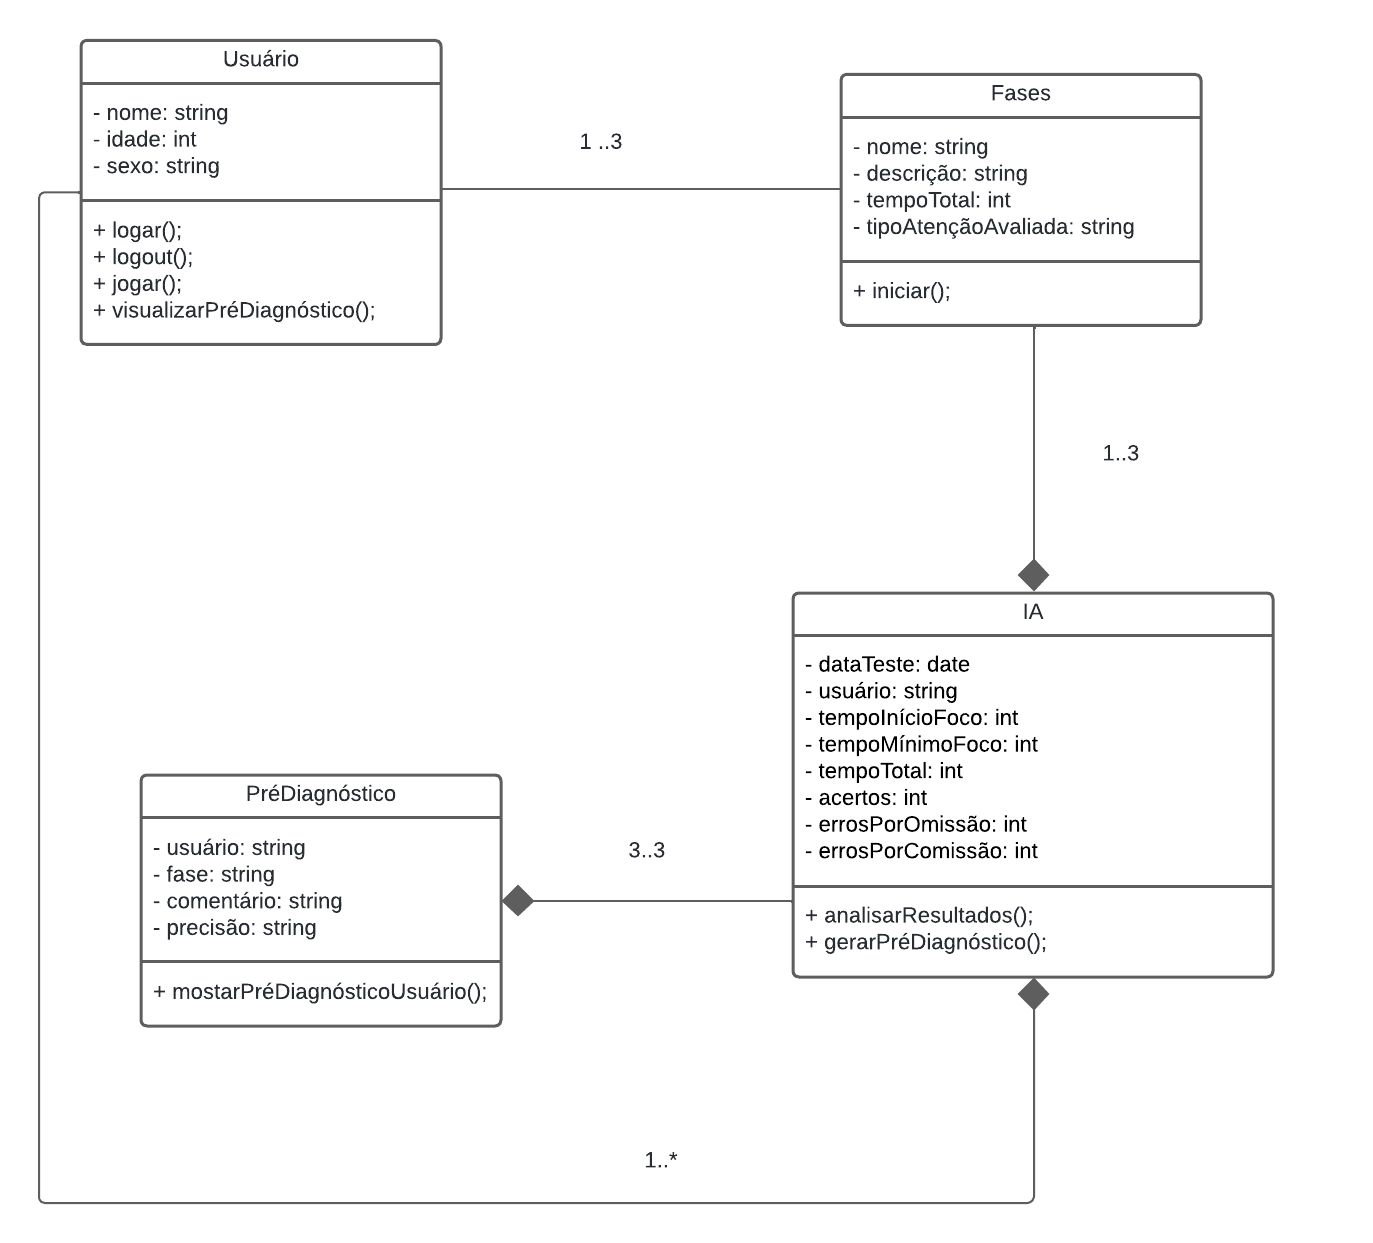
\includegraphics[width=0.8\textwidth]{Logos/diagrama-de-classe.png}
\SourceOrNote{Do próprio autor (2025)}
\end{figure}

     Não deixe a seção terminar com a imagem então sempre adicione um texto após a mesma.

    \subsection*{Diagrama de Objetos}
    \addcontentsline{toc}{section}{Diagrama de Objetos}

Esse é um exemplo de diagrama de objetos.

        \begin{figure}[H]
\centering
\caption{Diagrama de objetos}%
\label{fig:diagrama-de-objetos}
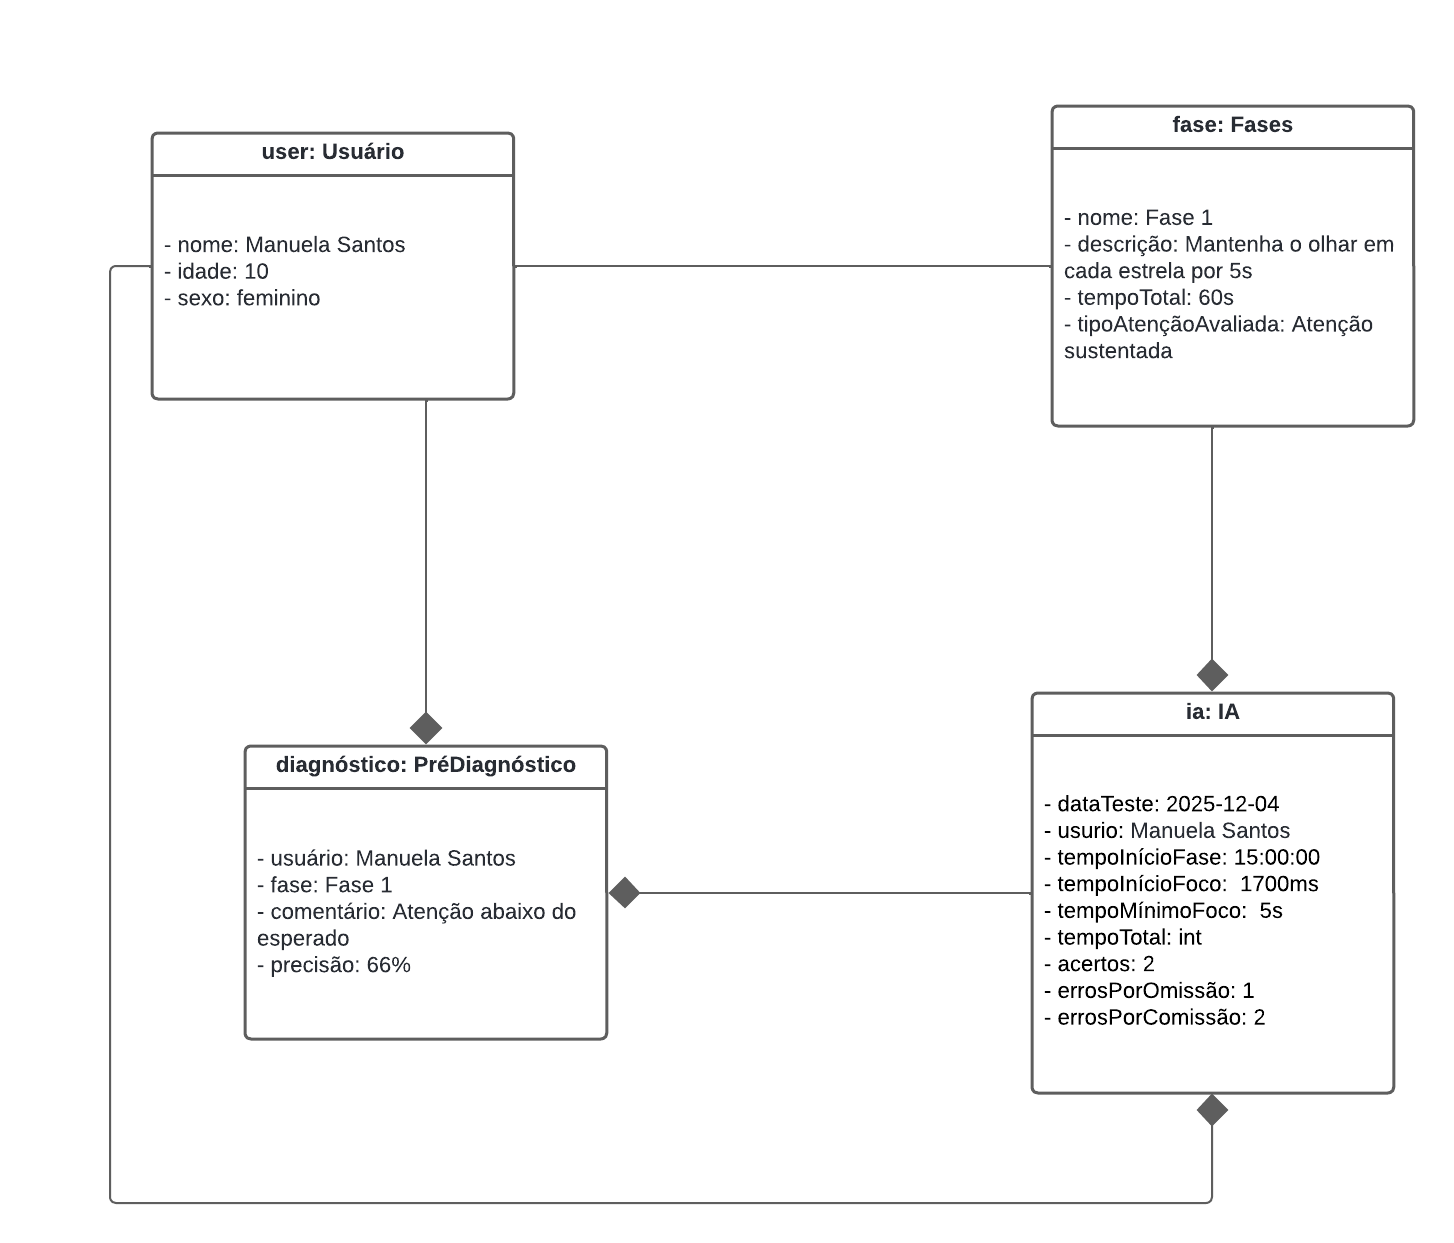
\includegraphics[width=0.8\textwidth]{Logos/diagrama-de-objetos.png}
\SourceOrNote{Do próprio autor (2025)}
\end{figure}

Não deixe a seção terminar com a imagem então sempre adicione um texto após a mesma.

% \section*{Diagrama de redes}
%     Esse é um exemplo de diagrama de redes, você deverá descrever todos os componentes presentes no diagrama (atores e funcionalidades do sistema).

% \begin{figure}[H]
% \centering
% \caption{Diagrama de redes}%
% \label{fig:diagrama-de-redes}
% 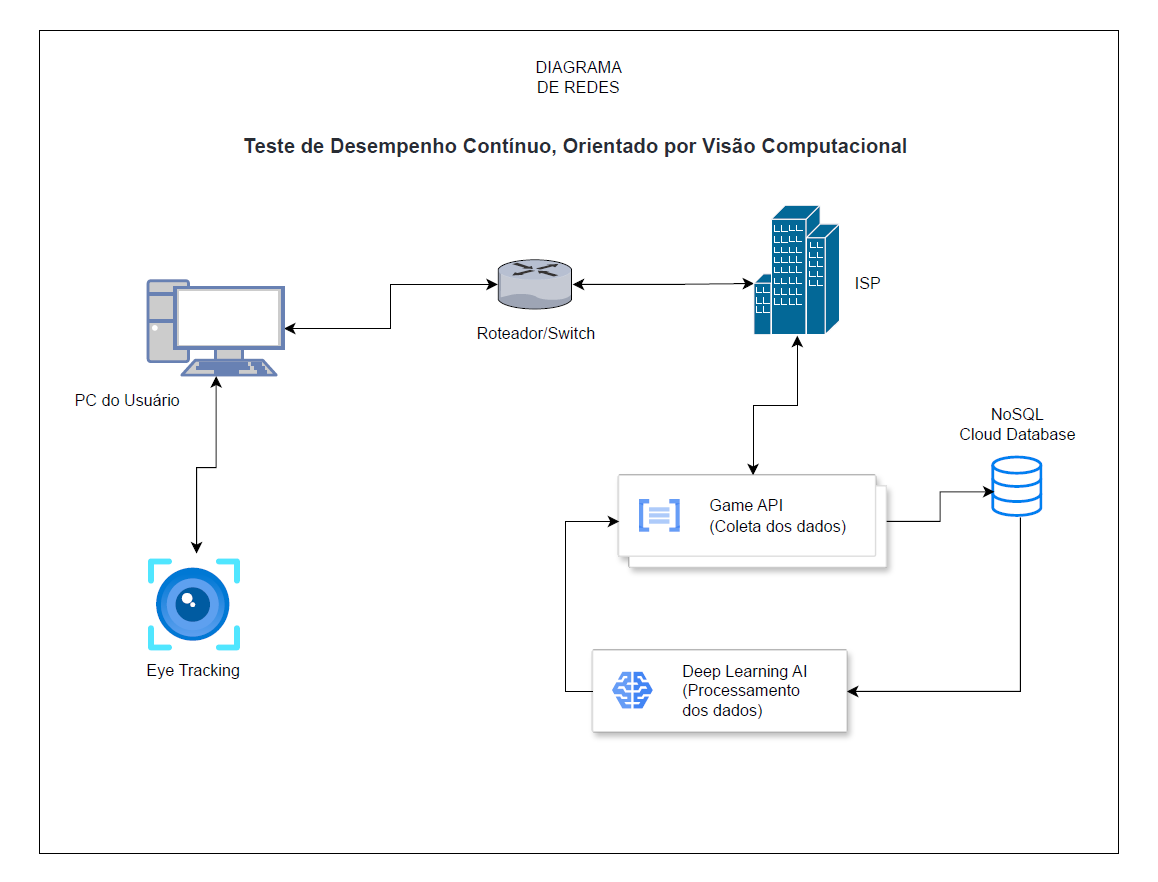
\includegraphics[width=1.1\textwidth]{Logos/diagrama-de-redes.png}
% \SourceOrNote{Do próprio autor (2025)}
% \end{figure}

%     Não deixe a seção terminar com a imagem então sempre adicione um texto após a mesma.

\end{document}